\documentclass[tikz, varwidth=540pt]{standalone}
\usepackage{amssymb, amsmath,bbm}

\standaloneenv{aaaa}

\begin{document}
	\begin{aaaa}
		\begin{center}	
		
		\fbox{%
			\begin{minipage}{0.90\linewidth}
				\centering
				\vspace{6pt}
		\tikzset{every picture/.style={line width=0.75pt}} %set default line width to 0.75pt        
		
		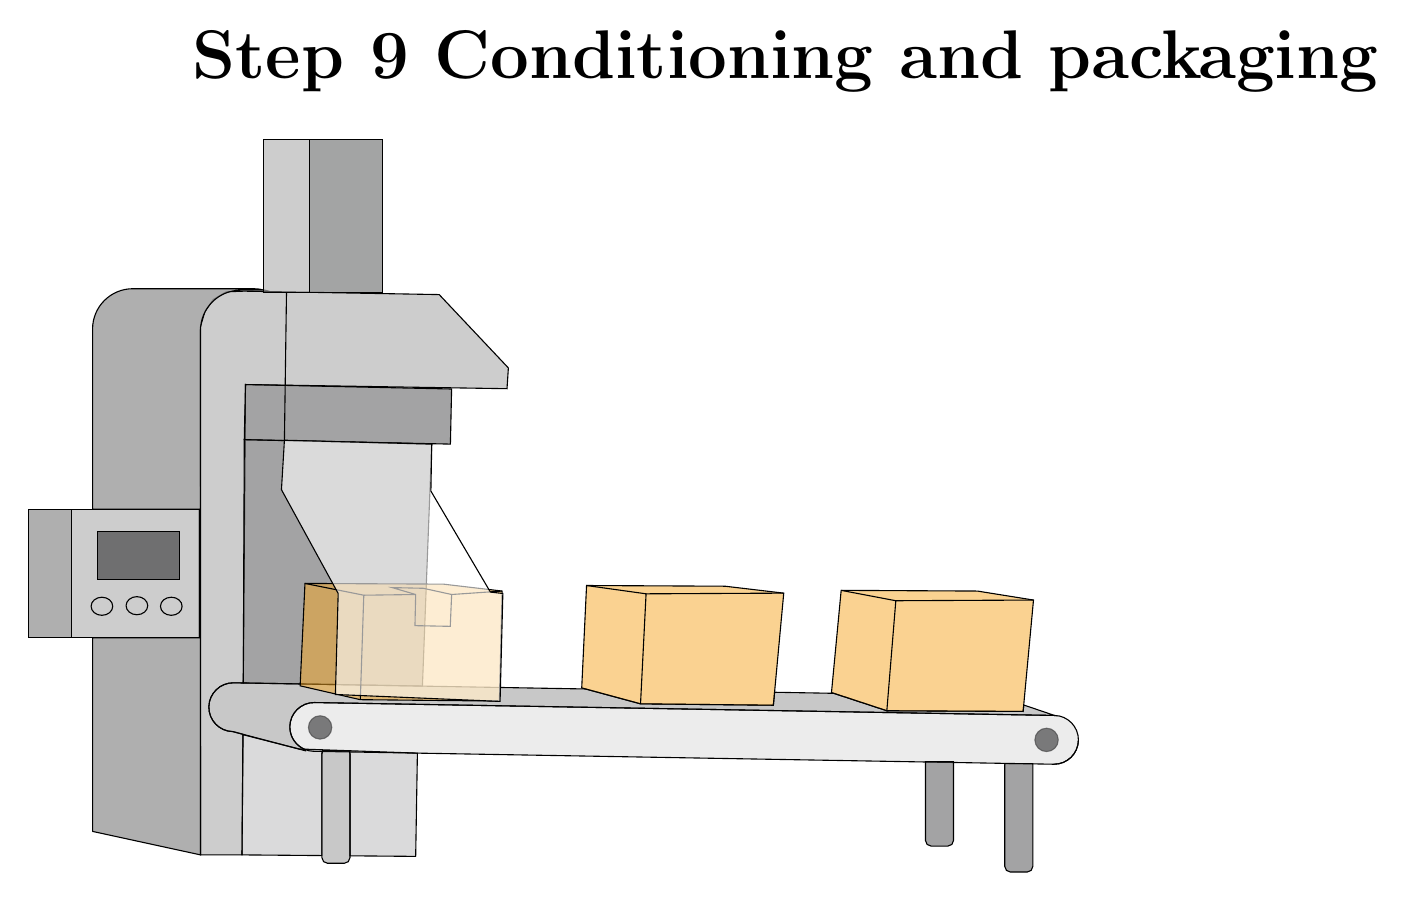
\begin{tikzpicture}[x=0.75pt,y=0.75pt,yscale=-1,xscale=1]
			%uncomment if require: \path (0,524); %set diagram left start at 0, and has height of 524
			
			%Shape: Path Data [id:dp7530417102908574] 
			\draw  [fill={rgb, 255:red, 155; green, 155; blue, 155 }  ,fill opacity=0.5 ] (307.14,141.43) -- (311.14,135.71) -- (317.43,132) -- (326,131.67) -- (420,133.33) -- (453.33,168.67) -- (452.67,178.67) -- (326.67,176.67) -- (325.61,320.46) -- (320.98,320.38) .. controls (314.49,320.27) and (309.14,325.44) .. (309.03,331.92) .. controls (308.92,338.41) and (314.08,343.76) .. (320.57,343.88) -- (325.43,345.16) -- (325,403.28) -- (305,403.28) -- (304.86,149.14) -- (307.14,141.43) -- cycle ;
			%Shape: Path Data [id:dp3831000191524848] 
			\draw  [fill={rgb, 255:red, 155; green, 155; blue, 155 }  ,fill opacity=0.8 ] (272.4,130.5) -- (330.6,130.5) .. controls (332.4,130.5) and (334.14,130.74) .. (335.79,131.2) -- (324.4,131.2) .. controls (313.69,131.2) and (305,139.89) .. (305,150.6) -- (305,403.28) -- (253.14,392) -- (253,391.86) -- (253,298.67) -- (304.33,298.67) -- (304.33,236.67) -- (253,236.67) -- (253,149.9) .. controls (253,139.19) and (261.69,130.5) .. (272.4,130.5) -- cycle ;
			%Shape: Path Data [id:dp2692110630299105] 
			\draw  [fill={rgb, 255:red, 72; green, 72; blue, 73 }  ,fill opacity=0.2 ] (325,403.28) -- (325.5,345.38) -- (352.5,352.25) -- (409.5,354.25) -- (408.67,404) -- (377,403.73) -- (377,354.52) .. controls (377,354.08) and (376.89,353.66) .. (376.7,353.29) -- (363.8,353.29) .. controls (363.61,353.66) and (363.5,354.08) .. (363.5,354.52) -- (363.5,403.61) -- (325,403.28) -- cycle ;
			%Shape: Rectangle [id:dp23715604466801987] 
			\draw  [fill={rgb, 255:red, 155; green, 155; blue, 155 }  ,fill opacity=0.8 ] (222,236.67) -- (242.67,236.67) -- (242.67,298.67) -- (222,298.67) -- cycle ;
			%Shape: Rectangle [id:dp26044959750762664] 
			\draw  [fill={rgb, 255:red, 155; green, 155; blue, 155 }  ,fill opacity=0.5 ] (242.67,236.67) -- (304.33,236.67) -- (304.33,298.67) -- (242.67,298.67) -- cycle ;
			%Shape: Rectangle [id:dp9912215442667679] 
			\draw  [fill={rgb, 255:red, 72; green, 72; blue, 73 }  ,fill opacity=0.7 ] (255.33,247.33) -- (294.67,247.33) -- (294.67,270.67) -- (255.33,270.67) -- cycle ;
			%Shape: Ellipse [id:dp18307260229647881] 
			\draw   (252.29,283.5) .. controls (252.29,281.09) and (254.62,279.14) .. (257.5,279.14) .. controls (260.38,279.14) and (262.71,281.09) .. (262.71,283.5) .. controls (262.71,285.91) and (260.38,287.86) .. (257.5,287.86) .. controls (254.62,287.86) and (252.29,285.91) .. (252.29,283.5) -- cycle ;
			%Shape: Ellipse [id:dp008436177237656106] 
			\draw   (269.14,283.21) .. controls (269.14,280.81) and (271.48,278.86) .. (274.36,278.86) .. controls (277.24,278.86) and (279.57,280.81) .. (279.57,283.21) .. controls (279.57,285.62) and (277.24,287.57) .. (274.36,287.57) .. controls (271.48,287.57) and (269.14,285.62) .. (269.14,283.21) -- cycle ;
			%Shape: Ellipse [id:dp7553515404676001] 
			\draw   (285.71,283.5) .. controls (285.71,281.09) and (288.05,279.14) .. (290.93,279.14) .. controls (293.81,279.14) and (296.14,281.09) .. (296.14,283.5) .. controls (296.14,285.91) and (293.81,287.86) .. (290.93,287.86) .. controls (288.05,287.86) and (285.71,285.91) .. (285.71,283.5) -- cycle ;
			%Shape: Rectangle [id:dp9457023922192831] 
			\draw  [fill={rgb, 255:red, 72; green, 73; blue, 73 }  ,fill opacity=0.5 ] (357.57,58.57) -- (392.57,58.57) -- (392.57,132.29) -- (357.57,132.29) -- cycle ;
			%Shape: Rectangle [id:dp853201411692196] 
			\draw  [fill={rgb, 255:red, 155; green, 155; blue, 155 }  ,fill opacity=0.5 ] (335.43,58.57) -- (357.57,58.57) -- (357.57,132.29) -- (335.43,132.29) -- cycle ;
			%Shape: Rectangle [id:dp1303638277346384] 
			\draw  [fill={rgb, 255:red, 72; green, 72; blue, 73 }  ,fill opacity=0.5 ] (326.67,176.67) -- (425.98,178.82) -- (425.4,205.37) -- (326.09,203.22) -- cycle ;
			%Straight Lines [id:da9889996233224269] 
			\draw    (346.43,132.49) -- (345.43,203.49) ;
			%Shape: Path Data [id:dp5764396545569709] 
			\draw  [fill={rgb, 255:red, 72; green, 72; blue, 73 }  ,fill opacity=0.5 ] (416.4,205.37) -- (411.92,321.95) -- (325.6,320.44) -- (326.09,203.22) -- (416.4,205.37) -- cycle ;
			%Rounded Rect [id:dp34951405327012985] 
			\draw  [fill={rgb, 255:red, 72; green, 72; blue, 73 }  ,fill opacity=0.1 ] (348.03,341.42) .. controls (348.14,334.94) and (353.49,329.77) .. (359.98,329.88) -- (716.43,336.1) .. controls (722.92,336.22) and (728.08,341.57) .. (727.97,348.06) -- (727.97,348.06) .. controls (727.86,354.54) and (722.51,359.71) .. (716.02,359.6) -- (359.57,353.38) .. controls (353.08,353.26) and (347.92,347.91) .. (348.03,341.42) -- cycle ;
			%Shape: Circle [id:dp25457581701894905] 
			\draw  [color={rgb, 255:red, 72; green, 72; blue, 73 }  ,draw opacity=0.7 ][fill={rgb, 255:red, 72; green, 72; blue, 73 }  ,fill opacity=0.7 ] (357,341.88) .. controls (357,338.77) and (359.52,336.25) .. (362.63,336.25) .. controls (365.73,336.25) and (368.25,338.77) .. (368.25,341.88) .. controls (368.25,344.98) and (365.73,347.5) .. (362.63,347.5) .. controls (359.52,347.5) and (357,344.98) .. (357,341.88) -- cycle ;
			%Shape: Circle [id:dp740828973634043] 
			\draw  [color={rgb, 255:red, 72; green, 72; blue, 73 }  ,draw opacity=0.7 ][fill={rgb, 255:red, 72; green, 72; blue, 73 }  ,fill opacity=0.7 ] (707,347.88) .. controls (707,344.77) and (709.52,342.25) .. (712.63,342.25) .. controls (715.73,342.25) and (718.25,344.77) .. (718.25,347.88) .. controls (718.25,350.98) and (715.73,353.5) .. (712.63,353.5) .. controls (709.52,353.5) and (707,350.98) .. (707,347.88) -- cycle ;
			%Shape: Path Data [id:dp18976370973143042] 
			\draw  [fill={rgb, 255:red, 72; green, 72; blue, 73 }  ,fill opacity=0.5 ] (667.79,358.74) -- (667.79,396.34) .. controls (667.79,397.83) and (666.58,399.04) .. (665.09,399.04) -- (656.99,399.04) .. controls (655.49,399.04) and (654.29,397.83) .. (654.29,396.34) -- (654.29,358.74) .. controls (654.29,358.63) and (654.29,358.53) .. (654.3,358.43) -- (667.77,358.43) .. controls (667.78,358.53) and (667.79,358.63) .. (667.79,358.74) -- cycle ;
			%Shape: Path Data [id:dp0034990849060657636] 
			\draw  [fill={rgb, 255:red, 72; green, 72; blue, 73 }  ,fill opacity=0.5 ] (706,359.74) -- (706,408.84) .. controls (706,410.33) and (704.79,411.54) .. (703.3,411.54) -- (695.2,411.54) .. controls (693.71,411.54) and (692.5,410.33) .. (692.5,408.84) -- (692.5,359.74) .. controls (692.5,359.59) and (692.51,359.44) .. (692.53,359.3) -- (705.97,359.3) .. controls (705.99,359.44) and (706,359.59) .. (706,359.74) -- cycle ;
			%Shape: Path Data [id:dp3602849072698926] 
			\draw  [fill={rgb, 255:red, 72; green, 72; blue, 73 }  ,fill opacity=0.3 ] (320.98,320.38) -- (490.54,323.34) -- (517,330.5) -- (581,331.17) -- (581.58,324.93) -- (610.1,325.43) -- (635.67,333.83) -- (701.33,334.17) -- (701.62,331.06) -- (716.43,336.1) -- (359.98,329.88) .. controls (353.49,329.77) and (348.14,334.94) .. (348.03,341.42) .. controls (347.94,346.54) and (351.14,350.96) .. (355.68,352.65) -- (355.64,353.14) -- (320.57,343.88) .. controls (314.08,343.76) and (308.92,338.41) .. (309.03,331.92) .. controls (309.14,325.44) and (314.49,320.27) .. (320.98,320.38) -- cycle (716.02,359.6) .. controls (722.51,359.71) and (727.86,354.54) .. (727.97,348.06) .. controls (727.86,354.54) and (722.51,359.71) .. (716.02,359.6) -- (716.02,359.6) -- cycle ;
			%Shape: Polygon [id:ds958229107808868] 
			\draw  [fill={rgb, 255:red, 245; green, 166; blue, 35 }  ,fill opacity=0.5 ] (557.67,273.83) -- (586,277.17) -- (581,331.17) -- (517,330.5) -- (488.67,322.83) -- (491,273.5) -- cycle ;
			%Shape: Polygon [id:ds10267683779694792] 
			\draw  [fill={rgb, 255:red, 245; green, 166; blue, 35 }  ,fill opacity=0.5 ] (706.33,280.5) -- (701.33,334.17) -- (635.67,333.83) -- (609,325.07) -- (613.67,275.83) -- (679.33,276.17) -- cycle ;
			%Straight Lines [id:da01989096100564347] 
			\draw    (491,273.5) -- (519.67,277.5) -- (517,330.5) ;
			%Straight Lines [id:da36216686785921337] 
			\draw    (519.67,277.5) -- (586,277.17) ;
			%Straight Lines [id:da3512795332003785] 
			\draw    (613.67,275.83) -- (640,280.83) -- (706.33,280.5) ;
			%Straight Lines [id:da18457983755931295] 
			\draw    (640,280.83) -- (635.67,333.83) ;
			%Shape: Polygon [id:ds27277028172254936] 
			\draw  [fill={rgb, 255:red, 245; green, 166; blue, 35 }  ,fill opacity=0.5 ] (422,272.83) -- (450.33,276.17) -- (449,329.17) -- (382,328.5) -- (353,321.83) -- (355.33,272.5) -- cycle ;
			%Straight Lines [id:da5306086221664243] 
			\draw    (355.33,272.5) -- (383.67,278.17) -- (382,328.5) ;
			%Straight Lines [id:da1607411024780938] 
			\draw    (383.67,278.17) -- (408.67,277.83) -- (408.33,292.83) -- (425.33,293.17) -- (426,277.83) -- (412.33,274.83) -- (397.33,274.5) -- (408.67,277.83) ;
			%Straight Lines [id:da5306076213613801] 
			\draw    (426,277.83) -- (450.33,276.17) ;
			%Shape: Polygon [id:ds9302610291582898] 
			\draw  [color={rgb, 255:red, 0; green, 0; blue, 0 }  ,draw opacity=1 ][fill={rgb, 255:red, 255; green, 255; blue, 255 }  ,fill opacity=0.6 ] (345.43,203.49) -- (416.4,205.37) -- (416,228) -- (444.67,276.67) -- (450.67,277.33) -- (449.33,329.33) -- (370,326) -- (371.33,277.33) -- (344,227.33) -- cycle ;
			%Shape: Path Data [id:dp7256278709844639] 
			\draw  [fill={rgb, 255:red, 72; green, 72; blue, 73 }  ,fill opacity=0.3 ] (377,354.52) -- (377,404.62) .. controls (377,406.11) and (375.79,407.32) .. (374.3,407.32) -- (366.2,407.32) .. controls (364.71,407.32) and (363.5,406.11) .. (363.5,404.62) -- (363.5,354.52) .. controls (363.5,354.08) and (363.61,353.66) .. (363.8,353.29) -- (376.7,353.29) .. controls (376.89,353.66) and (377,354.08) .. (377,354.52) -- cycle ;
			
			% Text Node
			\draw (300,5) node [anchor=north west][inner sep=0.75pt]  [font=\Huge] [align=left] {\textbf{Step 9 Conditioning and packaging}};
			
		\end{tikzpicture}
	    \vspace{6pt}
\end{minipage}}
		\end{center}
	\end{aaaa}
\end{document}